\chapter{फ़िल्टर और स्थानांतरण फलन}\label{ch:b1:filters-transfer-functions}

किसी ध्वनिविस्तारक की पेटी के भीतर एक कुंडली और एक संधारित्र, बिना किसी
ट्रांजिस्टर के, तय कर देते हैं कि मंद्र स्वर बड़े शंकु को जाएँ और तार स्वर छोटे
गुंबद को। किसी दोलनदर्शी का ``AC'' बटन धीरे-धीरे खिसकते किसी विस्थापन को हटा
देता है और उसके ऊपर की लहर रख लेता है। कोई विद्युत आपूर्ति एक ही संधारित्र से
धड़कती दिष्टकृत बिजली को स्थिर \omterm{def:b1:dc-circuits:voltage}{विभवांतर} बना देती है। तीनों \emph{\omterm{def:b1:filters-transfer-functions:H}{फ़िल्टर}} हैं:
यानी ऐसे \omterm{def:b1:dc-circuits:linear}{रैखिक परिपथ} जो हर आवृत्ति के साथ अलग बरताव करते हैं। चूँकि हर आवर्ती
संकेत ज्याओं का योग है, इसलिए यह जान लेना कि कोई परिपथ हर ज्या के साथ क्या
करता है --- यानी उसका \omterm{def:b1:filters-transfer-functions:H}{स्थानांतरण फलन} --- यह जान लेना है कि वह हर चीज़ के साथ
क्या करता है। यह अध्याय \omterm{def:b1:filters-transfer-functions:H}{स्थानांतरण फलन} परिभाषित करता है, पिछले अध्यायों के
प्रथम और द्वितीय कोटि के परिपथों के लिए उनके \omterm{def:b1:filters-transfer-functions:bode}{बोदे आरेख} खींचता है, और उनसे
अनुमान लगाता है कि कोई वर्ग तरंग \omterm{def:b1:filters-transfer-functions:H}{फ़िल्टर} से कैसी निकलती है।

\section{स्थानांतरण फलन और बोदे आरेख}

\begin{definition}[स्थानांतरण फलन]\label{def:b1:filters-transfer-functions:H}
\index{स्थानांतरण फलन}\index{लब्धि}\index{फ़िल्टर}
जिस \omterm{def:b1:dc-circuits:linear}{रैखिक परिपथ} का निवेश \omterm{def:b1:dc-circuits:voltage}{विभवांतर} $\underline U_e$ और निर्गम
\omterm{def:b1:dc-circuits:voltage}{विभवांतर} $\underline U_s$ हो (जो निर्गम पर कुछ भी जुड़े बिना लिया गया हो), उसका
\emph{स्थानांतरण फलन} है
\[
\underline H(j\omega) = \frac{\underline U_s}{\underline U_e},
\qquad G(\omega) = \abs{\underline H}, \qquad \varphi(\omega) = \arg\underline H,
\]
यानी \emph{लब्धि} $G$ (आयामों का अनुपात) और निवेश के सापेक्ष निर्गम का
कला-खिसकाव $\varphi$। \emph{फ़िल्टर} ऐसा ही परिपथ है, जिसे उसकी
आवृत्ति-निर्भरता के लिए काम में लिया जाता है: \omterm{def:b1:wave-propagation:signal}{आयाम} $E$ की कोई ज्या, $\omega$
पर, $G(\omega)E\cos(\omega t + \varphi(\omega))$ बनकर निकलती है।
\end{definition}

\begin{definition}[डेसिबल; बोदे आरेख]\label{def:b1:filters-transfer-functions:bode}
\index{डेसिबल}\index{बोदे आरेख}\index{कटऑफ़ आवृत्ति}\index{पारक बैंड}
\emph{डेसिबल} में \omterm{def:b1:filters-transfer-functions:H}{लब्धि} $G_{\mathrm{dB}} = 20\log_{10}G$ है: गुणक
$10$ यानी \qty{20}{dB}, गुणक $2$ यानी \qty{6}{dB}, और $1/\sqrt2$ यानी
\qty{-3}{dB}। \emph{बोदे आरेख} $G_{\mathrm{dB}}$ और
$\varphi$ को $\log_{10}\omega$ (या $f$) के सामने आलेखित करता है।
\emph{कटऑफ़ आवृत्ति} वहाँ है जहाँ $G$ गिरकर $G_{\max}/\sqrt2$ रह जाए
(अधिकतम से \qty{-3}{dB}); और \emph{पारक बैंड} आवृत्तियों का वह परास है जो
अधिकतम के \qty{3}{dB} के भीतर रहे। एक दशक आवृत्ति में गुणक $10$ है और
एक अष्टक गुणक $2$।
\end{definition}

\begin{method}[एक नज़र में फ़िल्टर की प्रकृति]\label{met:b1:filters-transfer-functions:nature}
गणना से पहले सीमाएँ देख लीजिए: बहुत कम आवृत्ति पर संधारित्र
खुला परिपथ होता है और कुंडली तार; और बहुत ऊँची आवृत्ति पर उलटा। हर एक को
बदलकर पढ़िए कि निर्गम निवेश ही है
(पार होता है) या शून्य (रुक जाता है)। कम को पार, ऊँचे को रोके: निम्न-पारक;
उलटा हो: उच्च-पारक; दोनों को रोके: बैंड-पारक; दोनों को पार करे: बैंड-रोधक।
फिर $\underline H$ को किसी \omterm{prop:b1:dc-circuits:dividers}{विभव विभाजक} से निकाल लीजिए।
\end{method}

\section{प्रथम कोटि के फ़िल्टर}

\begin{proposition}[प्रथम कोटि का निम्न-पारक]\label{prop:b1:filters-transfer-functions:lowpass1}
\index{निम्न-पारक फ़िल्टर}\index{समाकलक}
$C$ के आरपार निर्गम वाले RC विभाजक (या $R$ के आरपार निर्गम वाले RL
विभाजक) के लिए
\[
\underline H = \frac{1}{1 + j\omega/\omega_c}, \qquad
\omega_c = \frac{1}{RC} \ \Big(\text{या } \frac{R}{L}\Big),
\qquad G = \frac{1}{\sqrt{1 + (\omega/\omega_c)^2}}, \qquad
\varphi = -\arctan\frac{\omega}{\omega_c} .
\]
बोदे की अनंतस्पर्शियाँ: $G_{\mathrm{dB}} = 0$ जब $\omega \ll \omega_c$ हो, और
प्रति दशक \qty{20}{dB} गिरती एक सरल रेखा जब $\omega \gg \omega_c$ हो,
और वे $\omega_c$ पर मिलती हैं, जहाँ सच्चा वक्र \qty{-3}{dB} पर है और
$\varphi = -45^\circ$। $\omega \gg \omega_c$ के लिए $\underline H \approx
\omega_c/(j\omega)$: यानी निर्गम निवेश के \emph{समाकल} के समानुपाती होता है
--- वहाँ \omterm{def:b1:filters-transfer-functions:H}{फ़िल्टर} एक समाकलक है।
\end{proposition}

\begin{proof}
\omterm{prop:b1:dc-circuits:dividers}{विभव विभाजक}:
\[
\underline H = \frac{1/jC\omega}{R + 1/jC\omega} = \frac{1}{1 + jRC\omega} .
\]
कटऑफ़ से कहीं ऊपर $1 + j\omega/\omega_c \approx j\omega/\omega_c$, और
किसी \omterm{def:b1:sinusoidal-impedance:complex}{सम्मिश्र आयाम} को $j\omega$ से भाग देना समाकलन ही है
(\cref{prop:b1:sinusoidal-impedance:rules}): $u_s \approx \omega_c\int u_e\,\dd t$।
और $20\log(\omega_c/\omega)$ $\omega$ के हर दस गुने पर \qty{20}{dB} खोता है।
\end{proof}

\begin{proposition}[प्रथम कोटि का उच्च-पारक]\label{prop:b1:filters-transfer-functions:highpass1}
\index{उच्च-पारक फ़िल्टर}\index{अवकलक}
$R$ के आरपार निर्गम वाले CR विभाजक (या $L$ के आरपार निर्गम वाले LR) के
लिए
\[
\underline H = \frac{j\omega/\omega_c}{1 + j\omega/\omega_c},
\qquad G = \frac{\omega/\omega_c}{\sqrt{1 + (\omega/\omega_c)^2}},
\qquad \varphi = \frac{\pi}{2} - \arctan\frac{\omega}{\omega_c},
\]
जो $\omega_c$ से नीचे प्रति दशक \qty{20}{dB} चढ़ता है, ऊपर समतल रहता है, और
\qty{-3}{dB} तथा $+45^\circ$ देता है $\omega_c$ पर। $\omega \ll \omega_c$ के
लिए $\underline H
\approx j\omega/\omega_c$: यानी निर्गम निवेश के
\emph{अवकलज} के समानुपाती होता है।
\end{proposition}

\begin{proof}
$\underline H = R/(R + 1/jC\omega) = jRC\omega/(1 + jRC\omega)$;
और $j\omega$ से गुणा करना अवकलन ही है।
\end{proof}

\begin{omfigure}
\begin{tikzpicture}
\begin{axis}[omaxis, axis x line=bottom, axis y line=left, xlabel style={at={(axis description cs:0.5,-0.14)}, anchor=north}, width=7.4cm, height=5.2cm, xmode=log, xlabel={$\omega/\omega_c$},
    ylabel={$G_{\mathrm{dB}}$}, xmin=0.01, xmax=100, ymin=-42, ymax=6,
    ytick={0,-20,-40}, yticklabels={$0$,$-20$,$-40$},
    xtick={0.01,0.1,1,10,100}, xticklabels={$10^{-2}$,$10^{-1}$,$1$,$10$,$10^{2}$}]
  \addplot[omExo, dashed, domain=0.01:1, samples=2] {0};
  \addplot[omExo, dotted, domain=0.01:100, samples=2] {-3};
  \addplot[omExo, dashed, domain=1:100, samples=2] {-20*log10(x)};
  \addplot[omDef, thick, domain=0.01:100, samples=200] {-10*log10(1 + x^2)};
  \addplot[omThm, thick, domain=0.01:100, samples=200] {-10*log10(1 + 1/x^2)};
  \node[omDef, font=\footnotesize] at (axis cs:0.05,-7) {निम्न-पारक};
  \node[omThm, font=\footnotesize] at (axis cs:30,-9) {उच्च-पारक};
\end{axis}
\end{tikzpicture}\qquad
\begin{tikzpicture}
\begin{axis}[omaxis, axis x line=bottom, axis y line=left, xlabel style={at={(axis description cs:0.5,-0.14)}, anchor=north}, width=7.0cm, height=5.2cm, xmode=log, xlabel={$\omega/\omega_c$},
    ylabel={$\varphi$}, xmin=0.01, xmax=100, ymin=-1.8, ymax=1.8,
    ytick={-1.5708,-0.7854,0,0.7854,1.5708}, yticklabels={$-\frac{\pi}{2}$,$-\frac{\pi}{4}$,$0$,$\frac{\pi}{4}$,$\frac{\pi}{2}$},
    xtick={0.01,0.1,1,10,100}, xticklabels={$10^{-2}$,$10^{-1}$,$1$,$10$,$10^{2}$}]
  \addplot[omDef, thick, domain=0.01:100, samples=200] {-rad(atan(x))};
  \addplot[omThm, thick, domain=0.01:100, samples=200] {rad(90 - atan(x))};
\end{axis}
\end{tikzpicture}

{\small प्रथम कोटि के निम्न-पारक (नीला) और उच्च-पारक (लाल) के \omterm{def:b1:filters-transfer-functions:bode}{बोदे आरेख}:
\omterm{def:b1:filters-transfer-functions:bode}{डेसिबल} में \omterm{def:b1:filters-transfer-functions:H}{लब्धि}, जिसकी अनंतस्पर्शियाँ (बिंदुदार) कटऑफ़ पर मिलती हैं, जहाँ
सच्ची \omterm{def:b1:filters-transfer-functions:H}{लब्धि} \qty{-3}{dB} है, और \omterm{def:b1:wave-propagation:signal}{कला}, जो कटऑफ़ पर
$\mp45^\circ$ पार करती है।}
\end{omfigure}

\begin{example}[AC युग्मन]\label{ex:b1:filters-transfer-functions:accoupling}
किसी दोलनदर्शी का AC निवेश $f_c \approx \qty{10}{Hz}$ वाला उच्च-पारक है:
\qty{5}{V} के विस्थापन पर सवार \qty{1}{kHz} का संकेत
\qty{-0.0002}{dB} के साथ, अपना विस्थापन छोड़कर, पार हो जाता है। पर \qty{50}{Hz}
की वर्ग तरंग दिखाई देने लायक़ विकृत हो जाती है --- उसकी समतल चोटियाँ झुक जाती
हैं --- क्योंकि \qty{50}{Hz} पर \omterm{def:b1:filters-transfer-functions:H}{फ़िल्टर} अपने कटऑफ़ से केवल एक दशक ऊपर है और
संकेत के निचले संनादी \omterm{def:b1:wave-propagation:signal}{कला} में खिसक जाते हैं
(\cref{exo:b1:filters-transfer-functions:12})।
\end{example}

\section{द्वितीय कोटि के फ़िल्टर}

\begin{proposition}[तीन फ़िल्टरों के रूप में श्रेणी RLC]\label{prop:b1:filters-transfer-functions:rlc}
\index{बैंड-पारक फ़िल्टर}\index{द्वितीय कोटि का फ़िल्टर}
$x = \omega/\omega_0$, $\omega_0 = 1/\sqrt{LC}$ और $Q =
\sqrt{L/C}/R$ के साथ, $\underline U_e$ से खिलाया गया श्रेणी RLC, इस पर
निर्भर करते हुए कि निर्गम कहाँ से लिया जाए, देता है:
\begin{align*}
\text{निर्गम } C:&\quad \underline H = \frac{1}{1 - x^2 + jx/Q}, \\
\text{निर्गम } R:&\quad \underline H = \frac{jx/Q}{1 - x^2 + jx/Q} = \frac{1}{1 + jQ(x - 1/x)}, \\
\text{निर्गम } L:&\quad \underline H = \frac{-x^2}{1 - x^2 + jx/Q}:
\end{align*}
यानी द्वितीय कोटि का एक निम्न-पारक, एक बैंड-पारक और एक उच्च-पारक।
$\omega_0$ से दूर निम्न-पारक और उच्च-पारक प्रति दशक \qty{40}{dB} गिरते हैं,
और बैंड-पारक दोनों ओर प्रति दशक \qty{20}{dB}; बैंड-पारक
का अधिकतम $1$ $\omega_0$ पर है और उसकी बैंड-चौड़ाई $\Delta\omega =
\omega_0/Q$, जैसा \cref{thm:b1:sinusoidal-impedance:resonance} में था।
\end{proposition}

\begin{proof}
कुल \omterm{def:b1:sinusoidal-impedance:impedance}{प्रतिबाधा} $R + j(L\omega - 1/C\omega)$ के साथ \omterm{prop:b1:dc-circuits:dividers}{विभव विभाजक};
अंश और हर को $jC\omega$ से गुणा कीजिए और
$LC\omega_0^2 = 1$, $RC\omega_0 = 1/Q$ का उपयोग कीजिए। बैंड-पारक पिछले अध्याय
का धारा-अनुनाद ही है, जिसे $R$ के आरपार \omterm{def:b1:dc-circuits:voltage}{विभवांतर} के रूप में पढ़ा गया है।
\end{proof}

\begin{proposition}[द्वितीय कोटि का निम्न-पारक: $Q$ की भूमिका]\label{prop:b1:filters-transfer-functions:lowpass2}
\index{अनुनाद!फ़िल्टर का}
निम्न-पारक के लिए $G = 1/\sqrt{(1 - x^2)^2 + x^2/Q^2}$:
$Q > 1/\sqrt2$ के लिए \omterm{def:b1:filters-transfer-functions:H}{लब्धि} $1$ से ऊपर चढ़ जाती है, $\omega_0$ के पास (अनुनाद,
शिखर $\approx Q$ जब $Q$ बड़ा हो); $Q = 1/\sqrt2$ के लिए वह ``अधिकतम समतल''
होती है, $G = 1/\sqrt{1 + x^4}$, और $\omega_0$ पर ठीक \qty{-3}{dB}; और इससे
छोटे $Q$ के लिए वह पहले ही झुक जाती है। \omterm{def:b1:wave-propagation:signal}{कला} $0$ से $-\pi$ तक चलती है, और
$-\pi/2$ से गुज़रती है $\omega_0$ पर।
\end{proposition}

\begin{proof}
$(1 - x^2)^2 + x^2/Q^2 = 1 + x^4 + x^2(1/Q^2 - 2)$: बीच का पद
$Q^2 = \tfrac12$ के लिए लुप्त हो जाता है, उससे ऊपर ऋणात्मक (शिखर) और नीचे
धनात्मक (झुकाव); और $x = 1$ के पास का व्यवहार
\cref{prop:b1:sinusoidal-impedance:overvoltage} में देखा जा चुका है।
\end{proof}

\begin{omfigure}
\begin{tikzpicture}
\begin{axis}[omaxis, axis x line=bottom, axis y line=left, xlabel style={at={(axis description cs:0.5,-0.14)}, anchor=north}, width=7.4cm, height=5.4cm, xmode=log, xlabel={$\omega/\omega_0$},
    ylabel={$G_{\mathrm{dB}}$}, xmin=0.1, xmax=10, ymin=-45, ymax=15,
    ytick={10,0,-20,-40}, xtick={0.1,1,10}, xticklabels={$0.1$,$1$,$10$},
    legend style={at={(0.03,0.03)}, anchor=south west, font=\footnotesize, draw=none, fill=none}]
  \addplot[omDef, thick, domain=0.1:10, samples=300] {-10*log10((1 - x^2)^2 + x^2/9)};
  \addlegendentry{$Q = 3$}
  \addplot[omThm, thick, domain=0.1:10, samples=300] {-10*log10(1 + x^4)};
  \addlegendentry{$Q = 1/\sqrt2$}
  \addplot[omProp, thick, domain=0.1:10, samples=300] {-10*log10((1 - x^2)^2 + x^2/0.04)};
  \addlegendentry{$Q = 0.2$}
  \addplot[omExo, dashed, domain=1:10, samples=2] {-40*log10(x)};
\end{axis}
\end{tikzpicture}\qquad
\begin{tikzpicture}
\begin{axis}[omaxis, axis x line=bottom, axis y line=left, xlabel style={at={(axis description cs:0.5,-0.14)}, anchor=north}, width=7.0cm, height=5.4cm, xmode=log, xlabel={$\omega/\omega_0$},
    ylabel={$G_{\mathrm{dB}}$}, xmin=0.1, xmax=10, ymin=-45, ymax=5,
    ytick={0,-20,-40}, xtick={0.1,1,10}, xticklabels={$0.1$,$1$,$10$},
    legend style={at={(0.03,0.97)}, anchor=north west, font=\footnotesize, draw=none, fill=none}]
  \addplot[omExo, dotted, domain=0.1:10, samples=2, forget plot] {-3};
  \addplot[omDef, thick, domain=0.1:10, samples=400] {-10*log10(1 + 100*(x - 1/x)^2)};
  \addlegendentry{$Q = 10$}
  \addplot[omThm, thick, domain=0.1:10, samples=300] {-10*log10(1 + (x - 1/x)^2)};
  \addlegendentry{$Q = 1$}
\end{axis}
\end{tikzpicture}

{\small श्रेणी RLC से बने द्वितीय कोटि के \omterm{def:b1:filters-transfer-functions:H}{फ़िल्टर}। बाएँ, निम्न-पारक
($C$ के आरपार निर्गम) तीन $Q$ के लिए: एक अनुनाद-शिखर, अधिकतम समतल
अनुक्रिया, या पहले ही झुकाव, और तीनों \qty{-40}{dB} प्रति दशक वाली
अनंतस्पर्शी (बिंदुदार) से जा मिलते हैं। दाएँ, बैंड-पारक ($R$ के आरपार निर्गम):
चौड़ाई $\omega_0/Q$ का एक शिखर, जो दोनों ओर \qty{20}{dB} प्रति दशक गिरता है।}
\end{omfigure}

\begin{example}[एक क्रॉसओवर]\label{ex:b1:filters-transfer-functions:crossover}
किसी ध्वनिविस्तारक के वूफ़र और ट्वीटर, हर एक \qty{8}{\ohm} का, प्रवर्धक को
एक निम्न-पारक (श्रेणी में कुंडली) और एक उच्च-पारक (श्रेणी में
संधारित्र) के द्वारा साझा करते हैं, जो \qty{2}{kHz} पर कटे हैं: $L = R/\omega_c = \qty{0.64}{mH}$,
$C = 1/R\omega_c = \qty{10}{\micro F}$। \qty{2}{kHz} पर हर चालक इकाई को
\qty{-3}{dB} मिलते हैं, यानी आधी शक्ति, और हर आवृत्ति पर $G_L^2 + G_H^2 = 1$:
अतः शक्ति बँटती है, खोती नहीं। सप्ताहांत समस्या इसका और तीखा रूप गढ़ती है।
\end{example}

\section{किसी आवर्ती संकेत का फ़िल्टरन}

\begin{theorem}[फूरिये वियोजन]\label{thm:b1:filters-transfer-functions:fourier}
\index{फूरिये श्रेणी}\index{संनादी}\index{वर्णक्रम!आवर्ती संकेत का}
आवर्तकाल $T = 2\pi/\omega$ का कोई आवर्ती संकेत (यदि वह ठीक-ठाक नियमित हो)
किसी नियतांक और $\omega$ के गुणजों पर ज्याओं का योग होता है:
\[
s(t) = c_0 + \sum_{n = 1}^{\infty} c_n\cos(n\omega t + \varphi_n),
\]
जहाँ $c_0 = \langle s\rangle$ उसका औसत मान है; पद $n = 1$
\emph{मूल स्वर} है, बाक़ी \emph{संनादी}, और
\omterm{def:b1:wave-propagation:signal}{आयाम} $c_n$ मिलकर \emph{वर्णक्रम} बनाते हैं। \omterm{def:b1:wave-propagation:signal}{आयाम}
$\pm E$ की वर्ग तरंग के लिए $c_n = 4E/(n\pi)$ जब $n$ विषम हो, और $0$ जब $n$
सम हो; और \omterm{def:b1:wave-propagation:signal}{आयाम} $\pm E$ की त्रिभुज तरंग के लिए $c_n = 8E/(n\pi)^2$ जब $n$
विषम हो।
\end{theorem}
\admitted

\begin{remark}[इससे क्या लेना है]\label{rem:b1:filters-transfer-functions:fourier}
यह प्रमेय और $c_n$ की गणना वर्ष 2 के गणित के
पाठ्यक्रम की चीज़ें हैं। यहाँ यह एक औज़ार है: तीखे कोनों को बहुत सारे
संनादी चाहिए (वर्ग तरंग के केवल $1/n$ की तरह घटते हैं), और सहज संकेतों को
थोड़े ही (त्रिभुज के $1/n^2$ की तरह)। किसी संकेत की संनादी-सामग्री ही वह चीज़ है
जिससे किसी वाद्य की गुणता बनती है, और जिस पर \omterm{def:b1:filters-transfer-functions:H}{फ़िल्टर} काम करता है।
\end{remark}

\begin{proposition}[किसी आवर्ती संकेत का रैखिक फ़िल्टरन]\label{prop:b1:filters-transfer-functions:filtering}
\omterm{def:b1:filters-transfer-functions:H}{स्थानांतरण फलन} $\underline H$ वाले किसी \omterm{def:b1:filters-transfer-functions:H}{फ़िल्टर} से गुज़रकर प्रमेय का संकेत
बन जाता है
\[
s_{\text{निर्गम}}(t) = G(0)\,c_0 + \sum_{n \geq 1} G(n\omega)\,c_n\cos\!\big(n\omega t + \varphi_n + \varphi(n\omega)\big):
\]
यानी हर संनादी \emph{अपनी ही} आवृत्ति पर \omterm{def:b1:filters-transfer-functions:H}{लब्धि} से गुणित और \omterm{def:b1:wave-propagation:signal}{कला} से खिसकाया
जाता है, और फिर टुकड़े जोड़ दिए जाते हैं। अतः:
\begin{itemize}
  \item $\omega_c \ll \omega$ वाला निम्न-पारक मूलतः $c_0$ ही बचाता है:
        वह \emph{औसत} निकालता है (समतलन, तरंगिका हटाना), और किसी
        वर्ग तरंग को छोटी त्रिभुज तरंग बना देता है (समाकलन);
  \item $\omega_c \ll \omega$ वाला उच्च-पारक $c_0$ हटा देता है और बाक़ी को
        जाने देता है (AC युग्मन); और $\omega_c \gg \omega$ के साथ वह
        अवकलन करता है (वर्ग तरंग के किनारों पर नुकीली चोटियाँ);
  \item $n\omega$ पर सुर बिठाया, $Q \gg 1$ वाला बैंड-पारक अकेला
        $n$-वाँ संनादी छाँट लेता है: यानी वर्ग तरंग में से एक ज्या।
\end{itemize}
\end{proposition}

\begin{proof}
किसी \omterm{def:b1:dc-circuits:linear}{रैखिक परिपथ} के लिए अध्यारोपण (\cref{thm:b1:dc-circuits:superposition})
ज्यावक्रीय निवेशों के योग पर लगाया गया, और हर एक को
\cref{def:b1:filters-transfer-functions:H} से बरता गया।
\end{proof}

\begin{omfigure}
\begin{tikzpicture}
\begin{axis}[omaxis, axis x line=bottom, width=6.6cm, height=4.8cm, xlabel={संनादी $n$}, ylabel={$c_n/c_1$},
    xmin=0, xmax=10, ymin=0, ymax=1.15, xtick={1,3,5,7,9}, ytick={0.5,1}]
  \addplot[ybar, bar width=7pt, fill=omDef!35, draw=omDef] coordinates {(1,1) (3,0.333) (5,0.2) (7,0.143) (9,0.111)};
  \addplot[ybar, bar width=3.5pt, fill=omThm, draw=omThm] coordinates
    {(1,0.7071) (3,0.1054) (5,0.0392) (7,0.0202) (9,0.0123)};
  \node[omDef, font=\footnotesize] at (axis cs:6.0,0.9) {वर्ग तरंग (नीला)};
  \node[omThm, font=\footnotesize] at (axis cs:6.0,0.7) {निम्न-पारक के बाद (लाल)};
\end{axis}
\end{tikzpicture}\hfill
\begin{tikzpicture}
\begin{axis}[omaxis, axis x line=bottom, width=6.6cm, height=4.8cm, xlabel={$t/T$}, ylabel={$u$},
    xmin=0, xmax=2, ymin=-1.3, ymax=1.3, xtick={0.5,1,1.5,2}, ytick={-1,1}, yticklabels={$-E$,$E$}]
  % square wave
  \addplot[omDef!60, thick, const plot, domain=0:2, samples=5] coordinates {(0,1) (0.5,-1) (1,1) (1.5,-1) (2,-1)};
  % RC response with tau = T/(2pi) (wc = w): on each half period u = s + (u0 - s) e^{-t/tau}; steady amplitude A = tanh(T/(4 tau)) = tanh(pi/2)=0.917
  \addplot[omThm, thick, domain=0:0.5, samples=60] {1 - (1 + 0.917)*exp(-2*pi*x)};
  \addplot[omThm, thick, domain=0.5:1, samples=60] {-1 + (1 + 0.917)*exp(-2*pi*(x-0.5))};
  \addplot[omThm, thick, domain=1:1.5, samples=60] {1 - (1 + 0.917)*exp(-2*pi*(x-1))};
  \addplot[omThm, thick, domain=1.5:2, samples=60] {-1 + (1 + 0.917)*exp(-2*pi*(x-1.5))};
  % tau = T/(20 pi): wc = 10 w: amplitude tanh(5 pi)=1
  \addplot[omProp, thick, domain=0:0.5, samples=80] {1 - 2*exp(-20*pi*x)};
  \addplot[omProp, thick, domain=0.5:1, samples=80] {-1 + 2*exp(-20*pi*(x-0.5))};
  \addplot[omProp, thick, domain=1:1.5, samples=80] {1 - 2*exp(-20*pi*(x-1))};
  \addplot[omProp, thick, domain=1.5:2, samples=80] {-1 + 2*exp(-20*pi*(x-1.5))};
\end{axis}
\end{tikzpicture}

{\small प्रथम कोटि के निम्न-पारक से गुज़रती एक वर्ग तरंग। बाएँ: उसका
वर्णक्रम ($1/n$ में विषम संनादी) और मूल स्वर पर कटे \omterm{def:b1:filters-transfer-functions:H}{फ़िल्टर} के बाद का
वर्णक्रम। दाएँ: $\omega_c = \omega$ (लाल,
चरघातांकी चाप) और $\omega_c = 10\omega$ (नारंगी, केवल गोल कोने) के लिए
काल-संकेत; और $\omega_c \ll \omega$ के साथ निर्गम औसत के आसपास एक छोटी
त्रिभुज तरंग होता।}
\end{omfigure}

\begin{example}[आँकड़े]\label{ex:b1:filters-transfer-functions:numbers}
\omterm{def:b1:wave-propagation:signal}{आयाम} \qty{5}{V} की \qty{1}{kHz} वर्ग तरंग: \qty{1}{kHz} पर
\qty{6.37}{V}, \qty{3}{kHz} पर \qty{2.12}{V},
\qty{5}{kHz} पर \qty{1.27}{V} के संनादी। \qty{10}{Hz} पर कटे किसी RC
निम्न-पारक ($\tau = \qty{16}{ms}$) से गुज़रने पर निर्गम शून्य के आसपास
\omterm{def:b1:wave-propagation:signal}{आयाम} $ET/4\tau \approx \qty{80}{mV}$ की त्रिभुज तरंग होता है; और $Q = 20$ के
साथ \qty{3}{kHz} पर सुर बिठाए बैंड-पारक से गुज़रने पर \qty{3}{kHz} पर
\qty{2.1}{V} की ज्या, जिसमें पड़ोसियों का कुछ ही प्रतिशत बचता है
(\cref{exo:b1:filters-transfer-functions:8})।
\end{example}

\section{फ़िल्टरों का शृंखलन}

\begin{proposition}[शृंखलन और भार-प्रभाव]\label{prop:b1:filters-transfer-functions:cascade}
\index{शृंखलन (फ़िल्टरों का)}\index{भार-प्रभाव (फ़िल्टर पर)}
शृंखला में जुड़े दो फ़िल्टरों के लिए $\underline H = \underline H_1\underline H_2$
--- लब्धियाँ गुणित होती हैं, \omterm{def:b1:filters-transfer-functions:bode}{डेसिबल} और कलाएँ जुड़ती हैं --- \emph{बशर्ते दूसरा
पहले पर भार न डाले}, यानी उसके निर्गम से नगण्य धारा खींचे। अन्यथा विभाजक के
संबंध पूरे मिले-जुले जाल के लिए फिर से लिखने पड़ते हैं। चरणों के बीच लगा कोई
संक्रियात्मक-प्रवर्धक अनुगामी
(\cref{ch:b1:operational-amplifier}) गुणनफल के नियम को यथार्थ बना देता है।
\end{proposition}

\begin{proof}
$\underline H_1$ खुले निर्गम के साथ परिभाषित हुआ था; यदि अगले चरण की
निवेश \omterm{def:b1:sinusoidal-impedance:impedance}{प्रतिबाधा} पहले चरण की निर्गम \omterm{def:b1:sinusoidal-impedance:impedance}{प्रतिबाधा} (यानी उसके तेवेनिन प्रतिरोध)
से कहीं बड़ी हो, तो निर्गम \omterm{def:b1:dc-circuits:voltage}{विभवांतर} अपरिवर्तित रहता है और
दूसरा चरण अपने निवेश के रूप में ठीक $\underline U_{s1}$ देखता है।
\end{proof}

\begin{example}[दो RC चरण]\label{ex:b1:filters-transfer-functions:tworc}
पीठ-से-पीठ जुड़े दो एक जैसे RC निम्न-पारक
$1/(1 + j\omega/\omega_c)^2$ \emph{नहीं} देते: दूसरे चरण का $R$ पहले पर भार
डालता है। यथार्थ परिणाम $\underline H = 1/[1 - (\omega/\omega_c)^2 +
3j\omega/\omega_c]$ है, जो $\omega_c$ पर \qty{-9.5}{dB} है, न कि
\qty{-6}{dB} जिसका वादा गुणनफल का नियम करता है, हालाँकि दोनों आख़िर में उसी
\qty{-40}{dB} प्रति दशक ढाल तक पहुँचते हैं।
\end{example}

\section{अभ्यास}

\begin{exercise}[$\star$]\label{exo:b1:filters-transfer-functions:1}
\omterm{def:b1:filters-transfer-functions:bode}{डेसिबल} में बदलिए: लब्धियाँ $0.5$, $10$, $1/\sqrt2$, $100$। अनुपातों में
बदलिए: \qty{-40}{dB}, \qty{+6}{dB}। शृंखला में जुड़े दो \omterm{def:b1:filters-transfer-functions:H}{फ़िल्टर} (बिना भार के)
किसी आवृत्ति पर \qty{-6}{dB} और \qty{-20}{dB} देते हैं: कुल \omterm{def:b1:filters-transfer-functions:H}{लब्धि}?
\end{exercise}

\begin{exercise}[$\star$]\label{exo:b1:filters-transfer-functions:2}
RC निम्न-पारक, $R = \qty{10}{k\ohm}$, $C = \qty{16}{nF}$: \omterm{def:b1:filters-transfer-functions:bode}{कटऑफ़ आवृत्ति},
और \qty{100}{Hz}, \qty{1}{kHz}, \qty{10}{kHz},
\qty{100}{kHz} पर \omterm{def:b1:filters-transfer-functions:bode}{डेसिबल} में \omterm{def:b1:filters-transfer-functions:H}{लब्धि} निकालिए।
\end{exercise}

\begin{exercise}[$\star$]\label{exo:b1:filters-transfer-functions:3}
बिना गणना किए इनकी प्रकृति (निम्न-, उच्च-, बैंड-पारक) बताइए: (क)
श्रेणी में $R$, निर्गम के आरपार $C$; (ख) श्रेणी में $C$, निर्गम के आरपार
$R$; (ग) श्रेणी में $L$, निर्गम के आरपार $C$; (घ) श्रेणी में $L$ और $C$,
निर्गम के आरपार $R$।
\end{exercise}

\begin{exercise}[$\star$]\label{exo:b1:filters-transfer-functions:4}
\omterm{def:b1:wave-propagation:signal}{आयाम} \qty{5.0}{V} की \qty{1.0}{kHz} वर्ग तरंग: उसके पहले तीन अशून्य
संनादियों की आवृत्तियाँ और \omterm{def:b1:wave-propagation:signal}{आयाम} दीजिए। उसमें कोई सम संनादी क्यों नहीं है?
\end{exercise}

\begin{exercise}[$\star\star$]\label{exo:b1:filters-transfer-functions:5}
\qty{10}{kHz} पर कटा कोई CR उच्च-पारक \qty{100}{Hz} पर \omterm{def:b1:wave-propagation:signal}{आयाम}
\qty{1.0}{V} की त्रिभुज तरंग पाता है। समझाइए कि वह अवकलक की तरह क्यों बरतता
है और निर्गम की आकृति तथा \omterm{def:b1:wave-propagation:signal}{आयाम} दीजिए।
\end{exercise}

\begin{exercise}[$\star\star$]\label{exo:b1:filters-transfer-functions:6}
\qty{10}{Hz} पर कटा कोई RC निम्न-पारक \omterm{def:b1:wave-propagation:signal}{आयाम} $\pm\qty{1.0}{V}$ की \qty{1.0}{kHz}
वर्ग तरंग पाता है। दिखाइए कि निर्गम एक त्रिभुज तरंग है
और उसका \omterm{def:b1:wave-propagation:signal}{आयाम} निकालिए।
\end{exercise}

\begin{exercise}[$\star\star$]\label{exo:b1:filters-transfer-functions:7}
$L = \qty{10}{mH}$, $C = \qty{100}{nF}$ वाला कोई श्रेणी RLC निम्न-पारक:
$f_0$ दीजिए; अधिकतम समतल अनुक्रिया के लिए $R$ खोजिए; और $f_0$ पर तथा
$10f_0$ पर \omterm{def:b1:filters-transfer-functions:bode}{डेसिबल} में \omterm{def:b1:filters-transfer-functions:H}{लब्धि} दीजिए।
\end{exercise}

\begin{exercise}[$\star\star$]\label{exo:b1:filters-transfer-functions:8}
\qty{3.0}{kHz} पर सुर बिठाया कोई बैंड-पारक ($Q = 20$)
\cref{exo:b1:filters-transfer-functions:4} की \qty{1}{kHz} वर्ग तरंग पाता है।
$1$, $3$ और \qty{5}{kHz} पर \omterm{def:b1:filters-transfer-functions:H}{लब्धि}, और इन संनादियों के निर्गम \omterm{def:b1:wave-propagation:signal}{आयाम} निकालिए;
निर्गम का वर्णन कीजिए।
\end{exercise}

\begin{exercise}[$\star\star$]\label{exo:b1:filters-transfer-functions:9}
शृंखला में दो एक जैसे RC निम्न-पारक ($R = \qty{1.0}{k\ohm}$, $C = \qty{159}{nF}$)।
यथार्थ \omterm{def:b1:filters-transfer-functions:H}{स्थानांतरण फलन} (दूसरा पहले पर भार डालता है) और $\omega_c = 1/RC$ पर
\omterm{def:b1:filters-transfer-functions:H}{लब्धि} निकालिए; और अलग-अलग दोनों लब्धियों के गुणनफल से तुलना कीजिए।
\end{exercise}

\begin{exercise}[$\star\star\star$]\label{exo:b1:filters-transfer-functions:10}
$\underline H = (1 + j\omega/\omega_1)/
(1 + j\omega/\omega_2)$ की बोदे अनंतस्पर्शियाँ खींचिए, जहाँ $\omega_1 = \qty{100}{rad/s}$, $\omega_2 =
\qty{1e4}{rad/s}$: ढालें, कोने, \omterm{def:b1:filters-transfer-functions:bode}{डेसिबल} में ऊँची-आवृत्ति वाला पठार,
और $\sqrt{\omega_1\omega_2}$ पर \omterm{def:b1:wave-propagation:signal}{कला}।
\end{exercise}

\begin{exercise}[$\star\star\star$]\label{exo:b1:filters-transfer-functions:11}
पूर्ण-तरंग दिष्टकृत किसी ज्या (\qty{50}{Hz} की बिजली) का औसत $2E/\pi$ है और
\qty{100}{Hz} पर उसका पहला संनादी \omterm{def:b1:wave-propagation:signal}{आयाम} $4E/3\pi$ का। किसी RC
निम्न-पारक को \qty{100}{Hz} की तरंगिका को औसत के $1\%$ से नीचे लाना है:
आवश्यक \omterm{def:b1:filters-transfer-functions:bode}{कटऑफ़ आवृत्ति} और \omterm{def:b1:transient-regimes:firstorder}{कालांक} निकालिए। अकेला संधारित्र
(भार-प्रतिरोध के साथ) ही सामान्य चुनाव क्यों होता है?
\end{exercise}

\begin{exercise}[$\star\star\star$]\label{exo:b1:filters-transfer-functions:12}
किसी दोलनदर्शी का AC युग्मन $C = \qty{0.10}{\micro F}$
और $R = \qty{160}{k\ohm}$ वाला उच्च-पारक है। $f_c$ निकालिए। उस पर कोई वर्ग तरंग लगाई जाती है: दिखाइए
कि हर समतल चोटी एक क्षीण होता चरघातांक बन जाती है, और \qty{50}{Hz} पर तथा
\qty{1}{kHz} पर झोल (आधे आवर्तकाल में खोया अंश) निकालिए।
\end{exercise}

\begin{omfigure}
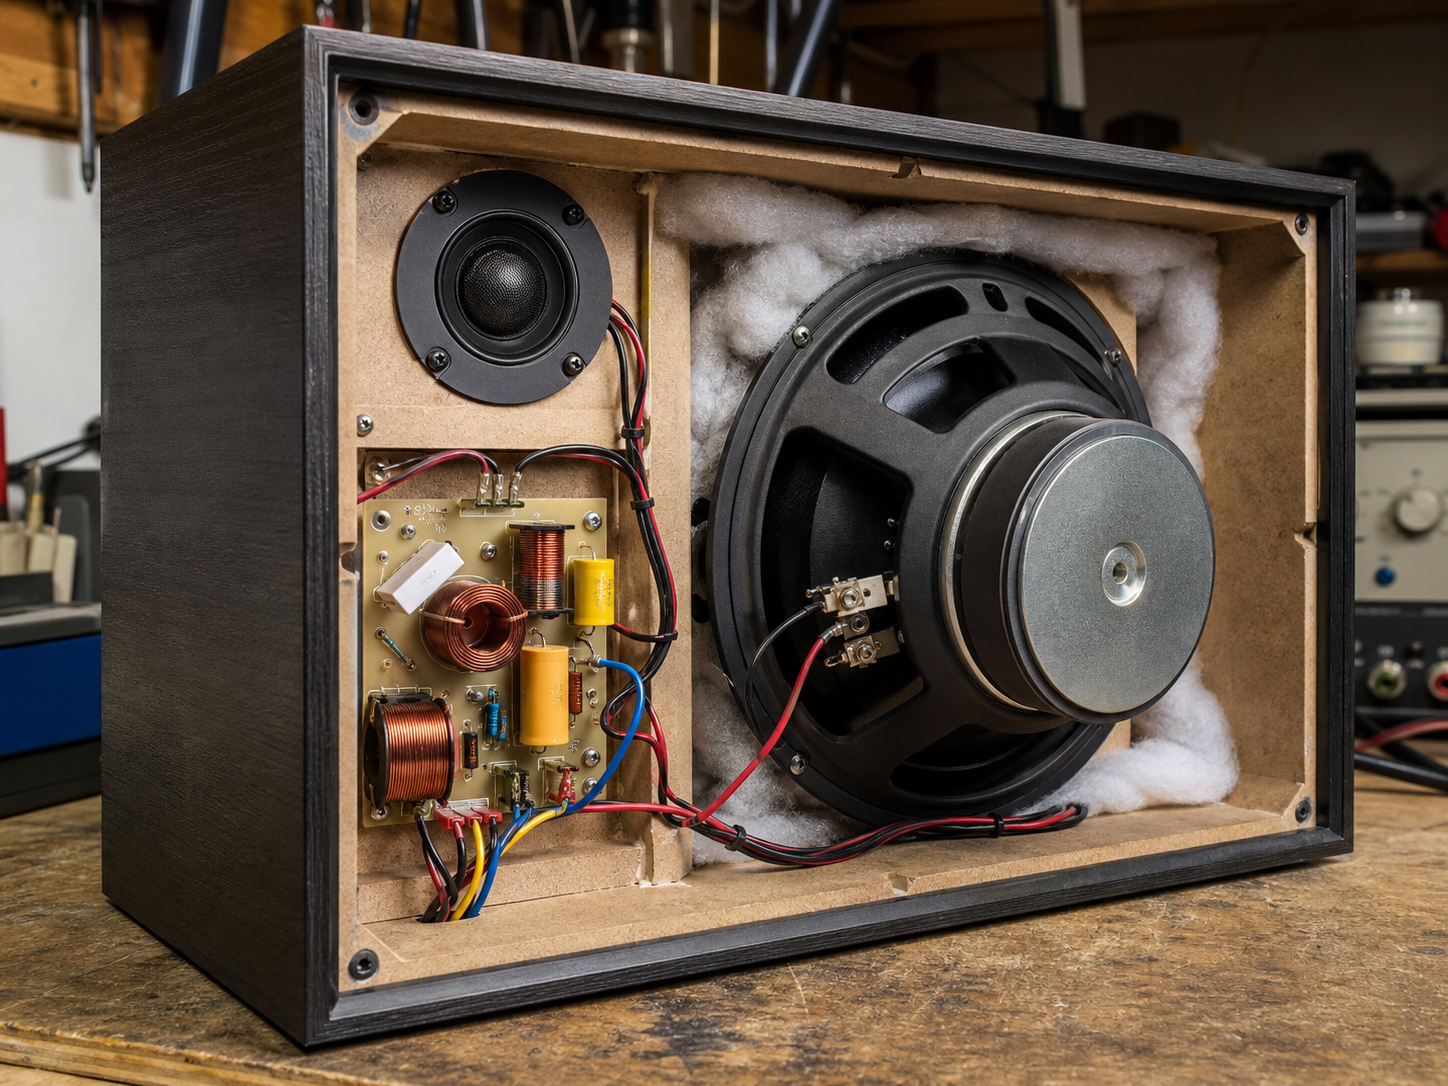
\includegraphics[width=0.50\linewidth]{images/book3/ai/b3-09-loudspeaker-crossover.png}

{\small दो-मार्गी ध्वनिविस्तारक के भीतर: क्रॉसओवर की कुंडलियाँ और संधारित्र ही वे निम्न-पारक और \omterm{prop:b1:filters-transfer-functions:highpass1}{उच्च-पारक फ़िल्टर} हैं जो मंद्र स्वर वूफ़र को और तार स्वर ट्वीटर को भेजते हैं।}
\end{omfigure}

\section{समस्या: ध्वनिविस्तारक का क्रॉसओवर}

\begin{problem}[{सप्ताहांत समस्या --- एक वूफ़र, एक ट्वीटर, एक कुंडली और एक
संधारित्र: कोई निष्क्रिय क्रॉसओवर संगीत को कैसे बाँटता है, सबसे सरल वाला
मंद्र स्वर ट्वीटर में क्यों रिसा देता है, और कोई असली ध्वनि-कुंडली अभिकल्पना
के साथ क्या करती है}]
\label{pb:b1:filters-transfer-functions:1}
वूफ़र और ट्वीटर को पहले शुद्ध प्रतिरोध
$R = \qty{8.0}{\ohm}$ मान लिया जाता है। प्रवर्धक एक आदर्श \omterm{def:b1:dc-circuits:sources}{विभव स्रोत}
$\underline U_e$ है। क्रॉसओवर आवृत्ति $f_c = \qty{2.0}{kHz}$ है।

\medskip
\noindent\textbf{भाग I --- प्रथम कोटि का क्रॉसओवर।}
वूफ़र को श्रेणी में जुड़ी कुंडली $L$ के द्वारा और ट्वीटर को श्रेणी में जुड़े
संधारित्र $C$ के द्वारा खिलाया जाता है।
\begin{enumerate}
  \item हर शाखा का \omterm{def:b1:filters-transfer-functions:H}{स्थानांतरण फलन} (चालक इकाई के आरपार \omterm{def:b1:dc-circuits:voltage}{विभवांतर} बटा
        $\underline U_e$) और \omterm{def:b1:filters-transfer-functions:bode}{डेसिबल} में \omterm{def:b1:filters-transfer-functions:H}{लब्धि} परिभाषित कीजिए।
  \item दिखाइए कि वूफ़र वाली शाखा प्रथम कोटि का निम्न-पारक है और उसका
        कटऑफ़ $\omega_c$ $R$ तथा $L$ के पदों में दीजिए।
  \item $L$ निकालिए, $f_c = \qty{2.0}{kHz}$ के लिए।
  \item दिखाइए कि ट्वीटर वाली शाखा प्रथम कोटि का उच्च-पारक है;
        $\omega_c$ दीजिए और $C$ निकालिए।
  \item $f_c$ पर, \qty{200}{Hz} पर और \qty{20}{kHz} पर हर चालक इकाई की
        \omterm{def:b1:filters-transfer-functions:H}{लब्धि} \omterm{def:b1:filters-transfer-functions:bode}{डेसिबल} में दीजिए।
  \item दिखाइए कि हर आवृत्ति पर $G_L^2 + G_H^2 = 1$। प्रवर्धक से खींची
        जाती शक्ति के लिए इसका क्या अर्थ है?
  \item $f_c$ पर हर शाखा की \omterm{def:b1:wave-propagation:signal}{कला} दीजिए; वहाँ दोनों
        चालक इकाइयों के \omterm{def:b1:dc-circuits:voltage}{विभवांतर} \omterm{def:b1:wave-propagation:signal}{कला} में कितना भिन्न हैं?
  \item $f_c$ से दूर दोनों अनुक्रियाओं की ढालें प्रति अष्टक \omterm{def:b1:filters-transfer-functions:bode}{डेसिबल} में
        क्या हैं?
\end{enumerate}

\medskip
\noindent\textbf{भाग II --- द्वितीय कोटि का क्रॉसओवर।}
अब वूफ़र को श्रेणी में जुड़ी कुंडली $L$ के द्वारा खिलाया जाता है, और चालक इकाई
के समांतर में एक संधारित्र $C$ लगा है।
\begin{enumerate}[resume]
  \item दिखाइए कि $\underline H = 1/(1 - LC\omega^2 + jL\omega/R)$।
  \item $\omega_0$ और $Q$ को $L$, $C$, $R$ के पदों में पहचानिए।
  \item $Q = 1/\sqrt2$ के लिए दिखाइए कि $G = 1/\sqrt{1 + (\omega/\omega_0)^4}$
        और यह कि \omterm{def:b1:filters-transfer-functions:H}{लब्धि} $\omega_0$ पर \qty{-3}{dB} है।
  \item $L$ तथा $C$ निकालिए, $f_0 = \qty{2.0}{kHz}$ और $Q = 1/\sqrt2$ के लिए।
  \item \qty{4}{kHz} और \qty{8}{kHz} पर \omterm{def:b1:filters-transfer-functions:bode}{डेसिबल} में \omterm{def:b1:filters-transfer-functions:H}{लब्धि} निकालिए;
        इससे प्रति अष्टक \omterm{def:b1:filters-transfer-functions:bode}{डेसिबल} में ढाल निकालिए।
  \item ट्वीटर वाली शाखा में $L$ और $C$ की भूमिकाएँ बदल जाती हैं (श्रेणी
        में $C$, समांतर में $L$): बिना नई गणना किए उसका \omterm{def:b1:filters-transfer-functions:H}{स्थानांतरण
        फलन} लिखिए।
  \item $f_0$ पर हर शाखा की \omterm{def:b1:wave-propagation:signal}{कला} निकालिए। ट्वीटर की तारों के साथ क्या करना
        पड़ेगा, और क्यों?
\end{enumerate}

\medskip
\noindent\textbf{भाग III --- क्रॉसओवर से गुज़रता संगीत।}
\begin{enumerate}[resume]
  \item \qty{220}{Hz} का कोई चेलो-स्वर 20वें तक के संनादी ढोता है।
        प्रथम कोटि के क्रॉसओवर के साथ कौन-से संनादी अधिकतर ट्वीटर को
        जाते हैं?
  \item नौवें संनादी का क्या होता है?
  \item परीक्षण-संकेत के रूप में \qty{1.0}{kHz} की वर्ग तरंग काम में ली
        जाती है। प्रथम कोटि के क्रॉसओवर के साथ उसके मूल स्वर, तीसरे और
        पाँचवें संनादी के लिए हर शाखा की \omterm{def:b1:filters-transfer-functions:H}{लब्धि} दीजिए।
  \item प्रवर्धक में ग़लती से \qty{1}{V} का दिष्ट विस्थापन आ जाता है। कौन-सी
        चालक इकाई सुरक्षित है, और किससे?
  \item प्रथम कोटि के क्रॉसओवर के साथ \qty{500}{Hz} के किसी स्वर के
        \omterm{def:b1:dc-circuits:voltage}{विभवांतर} का और शक्ति का कितना अंश ट्वीटर तक पहुँचता है?
        द्वितीय कोटि के साथ भी वही। ट्वीटर के बचे रहने के लिए यह क्यों
        मायने रखता है?
\end{enumerate}

\medskip
\noindent\textbf{भाग IV --- असली ध्वनि-कुंडली।}
वूफ़र असल में $R = \qty{8.0}{\ohm}$ है, जो ध्वनि-कुंडली के प्रेरकत्व
$L_{vc} = \qty{0.50}{mH}$ के साथ श्रेणी में है।
\begin{enumerate}[resume]
  \item \qty{2}{kHz} पर और \qty{8}{kHz} पर वूफ़र की \omterm{def:b1:sinusoidal-impedance:impedance}{प्रतिबाधा} (मापांक)
        निकालिए।
  \item इस \omterm{def:b1:sinusoidal-impedance:impedance}{प्रतिबाधा} के साथ \qty{2}{kHz} और \qty{8}{kHz} पर प्रथम कोटि
        वाली वूफ़र-लब्धि फिर से निकालिए, और आदर्श
        \qty{-3}{dB} तथा \qty{-12.3}{dB} से तुलना कीजिए। ढाल का क्या हुआ?
  \item कोई ``ज़ोबेल जाल'' --- $R_z = R$ के साथ श्रेणी में $C_z =
        L_{vc}/R^2$ --- वूफ़र के समांतर में जोड़ा जाता है। दिखाइए
        कि यह संयोजन हर आवृत्ति पर शुद्ध प्रतिरोध $R$ की तरह बरतता है,
        और $C_z$ निकालिए।
  \item प्रवर्धक \qty{8}{\ohm} में \qty{50}{W} देता है: यह कितना
        प्रभावी \omterm{def:b1:dc-circuits:voltage}{विभवांतर} है, और $f_c$ पर हर चालक इकाई को कितनी शक्ति
        मिलती है (प्रथम कोटि का क्रॉसओवर)? \qty{500}{Hz} पर ट्वीटर तक
        कितनी पहुँचती है?
  \item समझौतों का सार लिखिए: ढाल, \omterm{def:b1:wave-propagation:signal}{कला}, अवयवों की संख्या,
        ट्वीटर की सुरक्षा, और ज़ोबेल जाल की ज़रूरत।
\end{enumerate}
\end{problem}
